% Created by tikzDevice version 0.11 on 2018-05-23 09:42:09
% !TEX encoding = UTF-8 Unicode
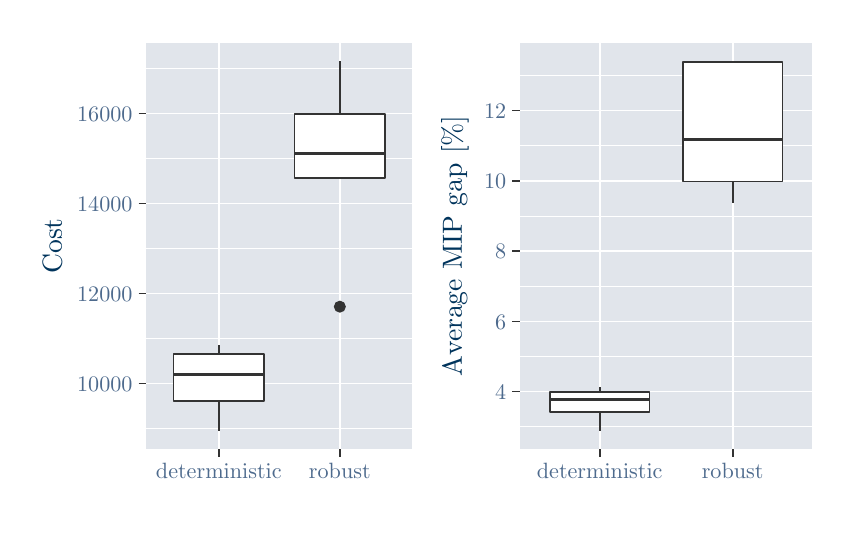
\begin{tikzpicture}[x=1pt,y=1pt]
\definecolor{fillColor}{RGB}{255,255,255}
\path[use as bounding box,fill=fillColor,fill opacity=0.00] (0,0) rectangle (289.08,180.67);
\begin{scope}
\path[clip] (  0.00,  0.00) rectangle (144.54,180.67);
\definecolor{drawColor}{RGB}{255,255,255}
\definecolor{fillColor}{RGB}{255,255,255}

\path[draw=drawColor,line width= 0.6pt,line join=round,line cap=round,fill=fillColor] (  0.00,  0.00) rectangle (144.54,180.68);
\end{scope}
\begin{scope}
\path[clip] ( 42.83, 28.35) rectangle (139.04,175.17);
\definecolor{fillColor}{RGB}{225,229,235}

\path[fill=fillColor] ( 42.83, 28.35) rectangle (139.04,175.17);
\definecolor{drawColor}{RGB}{255,255,255}

\path[draw=drawColor,line width= 0.3pt,line join=round] ( 42.83, 35.88) --
	(139.04, 35.88);

\path[draw=drawColor,line width= 0.3pt,line join=round] ( 42.83, 68.37) --
	(139.04, 68.37);

\path[draw=drawColor,line width= 0.3pt,line join=round] ( 42.83,100.86) --
	(139.04,100.86);

\path[draw=drawColor,line width= 0.3pt,line join=round] ( 42.83,133.35) --
	(139.04,133.35);

\path[draw=drawColor,line width= 0.3pt,line join=round] ( 42.83,165.84) --
	(139.04,165.84);

\path[draw=drawColor,line width= 0.6pt,line join=round] ( 42.83, 52.13) --
	(139.04, 52.13);

\path[draw=drawColor,line width= 0.6pt,line join=round] ( 42.83, 84.62) --
	(139.04, 84.62);

\path[draw=drawColor,line width= 0.6pt,line join=round] ( 42.83,117.11) --
	(139.04,117.11);

\path[draw=drawColor,line width= 0.6pt,line join=round] ( 42.83,149.60) --
	(139.04,149.60);

\path[draw=drawColor,line width= 0.6pt,line join=round] ( 69.07, 28.35) --
	( 69.07,175.17);

\path[draw=drawColor,line width= 0.6pt,line join=round] (112.80, 28.35) --
	(112.80,175.17);
\definecolor{drawColor}{gray}{0.20}

\path[draw=drawColor,line width= 0.6pt,line join=round] ( 69.07, 62.81) -- ( 69.07, 65.92);

\path[draw=drawColor,line width= 0.6pt,line join=round] ( 69.07, 45.65) -- ( 69.07, 35.02);
\definecolor{fillColor}{RGB}{255,255,255}

\path[draw=drawColor,line width= 0.6pt,line join=round,line cap=round,fill=fillColor] ( 52.67, 62.81) --
	( 52.67, 45.65) --
	( 85.47, 45.65) --
	( 85.47, 62.81) --
	( 52.67, 62.81) --
	cycle;

\path[draw=drawColor,line width= 1.1pt,line join=round] ( 52.67, 55.48) -- ( 85.47, 55.48);
\definecolor{fillColor}{gray}{0.20}

\path[draw=drawColor,line width= 0.4pt,line join=round,line cap=round,fill=fillColor] (112.80, 79.85) circle (  1.96);

\path[draw=drawColor,line width= 0.6pt,line join=round] (112.80,149.47) -- (112.80,168.50);

\path[draw=drawColor,line width= 0.6pt,line join=round] (112.80,126.45) -- (112.80,126.45);
\definecolor{fillColor}{RGB}{255,255,255}

\path[draw=drawColor,line width= 0.6pt,line join=round,line cap=round,fill=fillColor] ( 96.40,149.47) --
	( 96.40,126.45) --
	(129.20,126.45) --
	(129.20,149.47) --
	( 96.40,149.47) --
	cycle;

\path[draw=drawColor,line width= 1.1pt,line join=round] ( 96.40,135.32) -- (129.20,135.32);
\end{scope}
\begin{scope}
\path[clip] (  0.00,  0.00) rectangle (289.08,180.67);
\definecolor{drawColor}{RGB}{77,106,141}

\node[text=drawColor,anchor=base east,inner sep=0pt, outer sep=0pt, scale=  0.80] at ( 37.88, 49.37) {10000};

\node[text=drawColor,anchor=base east,inner sep=0pt, outer sep=0pt, scale=  0.80] at ( 37.88, 81.86) {12000};

\node[text=drawColor,anchor=base east,inner sep=0pt, outer sep=0pt, scale=  0.80] at ( 37.88,114.35) {14000};

\node[text=drawColor,anchor=base east,inner sep=0pt, outer sep=0pt, scale=  0.80] at ( 37.88,146.84) {16000};
\end{scope}
\begin{scope}
\path[clip] (  0.00,  0.00) rectangle (289.08,180.67);
\definecolor{drawColor}{gray}{0.20}

\path[draw=drawColor,line width= 0.6pt,line join=round] ( 40.08, 52.13) --
	( 42.83, 52.13);

\path[draw=drawColor,line width= 0.6pt,line join=round] ( 40.08, 84.62) --
	( 42.83, 84.62);

\path[draw=drawColor,line width= 0.6pt,line join=round] ( 40.08,117.11) --
	( 42.83,117.11);

\path[draw=drawColor,line width= 0.6pt,line join=round] ( 40.08,149.60) --
	( 42.83,149.60);
\end{scope}
\begin{scope}
\path[clip] (  0.00,  0.00) rectangle (289.08,180.67);
\definecolor{drawColor}{gray}{0.20}

\path[draw=drawColor,line width= 0.6pt,line join=round] ( 69.07, 25.60) --
	( 69.07, 28.35);

\path[draw=drawColor,line width= 0.6pt,line join=round] (112.80, 25.60) --
	(112.80, 28.35);
\end{scope}
\begin{scope}
\path[clip] (  0.00,  0.00) rectangle (289.08,180.67);
\definecolor{drawColor}{RGB}{77,106,141}

\node[text=drawColor,anchor=base,inner sep=0pt, outer sep=0pt, scale=  0.80] at ( 69.07, 17.89) {deterministic};

\node[text=drawColor,anchor=base,inner sep=0pt, outer sep=0pt, scale=  0.80] at (112.80, 17.89) {robust};
\end{scope}
\begin{scope}
\path[clip] (  0.00,  0.00) rectangle (289.08,180.67);
\definecolor{drawColor}{RGB}{0,52,92}

\node[text=drawColor,rotate= 90.00,anchor=base,inner sep=0pt, outer sep=0pt, scale=  1.00] at ( 12.39,101.76) {Cost};
\end{scope}
\begin{scope}
\path[clip] (144.54,  0.00) rectangle (289.08,180.67);
\definecolor{drawColor}{RGB}{255,255,255}
\definecolor{fillColor}{RGB}{255,255,255}

\path[draw=drawColor,line width= 0.6pt,line join=round,line cap=round,fill=fillColor] (144.54,  0.00) rectangle (289.08,180.68);
\end{scope}
\begin{scope}
\path[clip] (177.87, 28.35) rectangle (283.58,175.17);
\definecolor{fillColor}{RGB}{225,229,235}

\path[fill=fillColor] (177.87, 28.35) rectangle (283.58,175.17);
\definecolor{drawColor}{RGB}{255,255,255}

\path[draw=drawColor,line width= 0.3pt,line join=round] (177.87, 36.44) --
	(283.58, 36.44);

\path[draw=drawColor,line width= 0.3pt,line join=round] (177.87, 61.84) --
	(283.58, 61.84);

\path[draw=drawColor,line width= 0.3pt,line join=round] (177.87, 87.24) --
	(283.58, 87.24);

\path[draw=drawColor,line width= 0.3pt,line join=round] (177.87,112.64) --
	(283.58,112.64);

\path[draw=drawColor,line width= 0.3pt,line join=round] (177.87,138.05) --
	(283.58,138.05);

\path[draw=drawColor,line width= 0.3pt,line join=round] (177.87,163.45) --
	(283.58,163.45);

\path[draw=drawColor,line width= 0.6pt,line join=round] (177.87, 49.14) --
	(283.58, 49.14);

\path[draw=drawColor,line width= 0.6pt,line join=round] (177.87, 74.54) --
	(283.58, 74.54);

\path[draw=drawColor,line width= 0.6pt,line join=round] (177.87, 99.94) --
	(283.58, 99.94);

\path[draw=drawColor,line width= 0.6pt,line join=round] (177.87,125.35) --
	(283.58,125.35);

\path[draw=drawColor,line width= 0.6pt,line join=round] (177.87,150.75) --
	(283.58,150.75);

\path[draw=drawColor,line width= 0.6pt,line join=round] (206.70, 28.35) --
	(206.70,175.17);

\path[draw=drawColor,line width= 0.6pt,line join=round] (254.75, 28.35) --
	(254.75,175.17);
\definecolor{drawColor}{gray}{0.20}

\path[draw=drawColor,line width= 0.6pt,line join=round] (206.70, 49.02) -- (206.70, 50.90);

\path[draw=drawColor,line width= 0.6pt,line join=round] (206.70, 41.69) -- (206.70, 35.02);
\definecolor{fillColor}{RGB}{255,255,255}

\path[draw=drawColor,line width= 0.6pt,line join=round,line cap=round,fill=fillColor] (188.69, 49.02) --
	(188.69, 41.69) --
	(224.72, 41.69) --
	(224.72, 49.02) --
	(188.69, 49.02) --
	cycle;

\path[draw=drawColor,line width= 1.1pt,line join=round] (188.69, 46.15) -- (224.72, 46.15);

\path[draw=drawColor,line width= 0.6pt,line join=round] (254.75,168.31) -- (254.75,168.50);

\path[draw=drawColor,line width= 0.6pt,line join=round] (254.75,125.08) -- (254.75,117.49);

\path[draw=drawColor,line width= 0.6pt,line join=round,line cap=round,fill=fillColor] (236.73,168.31) --
	(236.73,125.08) --
	(272.77,125.08) --
	(272.77,168.31) --
	(236.73,168.31) --
	cycle;

\path[draw=drawColor,line width= 1.1pt,line join=round] (236.73,140.32) -- (272.77,140.32);
\end{scope}
\begin{scope}
\path[clip] (  0.00,  0.00) rectangle (289.08,180.67);
\definecolor{drawColor}{RGB}{77,106,141}

\node[text=drawColor,anchor=base east,inner sep=0pt, outer sep=0pt, scale=  0.80] at (172.92, 46.38) {4};

\node[text=drawColor,anchor=base east,inner sep=0pt, outer sep=0pt, scale=  0.80] at (172.92, 71.78) {6};

\node[text=drawColor,anchor=base east,inner sep=0pt, outer sep=0pt, scale=  0.80] at (172.92, 97.19) {8};

\node[text=drawColor,anchor=base east,inner sep=0pt, outer sep=0pt, scale=  0.80] at (172.92,122.59) {10};

\node[text=drawColor,anchor=base east,inner sep=0pt, outer sep=0pt, scale=  0.80] at (172.92,147.99) {12};
\end{scope}
\begin{scope}
\path[clip] (  0.00,  0.00) rectangle (289.08,180.67);
\definecolor{drawColor}{gray}{0.20}

\path[draw=drawColor,line width= 0.6pt,line join=round] (175.12, 49.14) --
	(177.87, 49.14);

\path[draw=drawColor,line width= 0.6pt,line join=round] (175.12, 74.54) --
	(177.87, 74.54);

\path[draw=drawColor,line width= 0.6pt,line join=round] (175.12, 99.94) --
	(177.87, 99.94);

\path[draw=drawColor,line width= 0.6pt,line join=round] (175.12,125.35) --
	(177.87,125.35);

\path[draw=drawColor,line width= 0.6pt,line join=round] (175.12,150.75) --
	(177.87,150.75);
\end{scope}
\begin{scope}
\path[clip] (  0.00,  0.00) rectangle (289.08,180.67);
\definecolor{drawColor}{gray}{0.20}

\path[draw=drawColor,line width= 0.6pt,line join=round] (206.70, 25.60) --
	(206.70, 28.35);

\path[draw=drawColor,line width= 0.6pt,line join=round] (254.75, 25.60) --
	(254.75, 28.35);
\end{scope}
\begin{scope}
\path[clip] (  0.00,  0.00) rectangle (289.08,180.67);
\definecolor{drawColor}{RGB}{77,106,141}

\node[text=drawColor,anchor=base,inner sep=0pt, outer sep=0pt, scale=  0.80] at (206.70, 17.89) {deterministic};

\node[text=drawColor,anchor=base,inner sep=0pt, outer sep=0pt, scale=  0.80] at (254.75, 17.89) {robust};
\end{scope}
\begin{scope}
\path[clip] (  0.00,  0.00) rectangle (289.08,180.67);
\definecolor{drawColor}{RGB}{0,52,92}

\node[text=drawColor,rotate= 90.00,anchor=base,inner sep=0pt, outer sep=0pt, scale=  1.00] at (156.93,101.76) {Average MIP gap [\%]};
\end{scope}
\end{tikzpicture}
